\documentclass{article}
\usepackage[margin=1in]{geometry}
\usepackage{enumitem}
\usepackage{setspace}
\usepackage{amsmath}
\usepackage{amssymb}
\usepackage{physics}
\usepackage{graphicx}

\title{Math 132 Homework 1}
\date{10/16/2020}
\author{Jiaping Zeng}

\begin{document}
\setstretch{1.35}
\maketitle

\begin{itemize}
    \item [1.1.5] $(\overline{2-i})^2$\\
          \textbf{Answer: } $(\overline{2-i})^2=(2+i)^2=4+4i-1=3+4i$
    \item [1.1.7] $(x+iy)^2$\\
          \textbf{Answer: } $(x+iy)^2=x^2+2xyi-y^2=(x^2-y^2)+i(2xy)$
    \item [1.1.8] $i\overline{(2+i)^2}$\\
          \textbf{Answer: } $i\overline{(2+i)^2}=i\overline{3+4i}=i(3-4i)=4+3i$
    \item [1.2.10] $\abs{\overline{(2+3i)^8}}$\\
          \textbf{Answer: } $\abs{\overline{(2+3i)^8}}=\abs{(2+3i)^8}=\abs{2+3i}^8=\sqrt{13}^8=13^4=28561$
    \item [1.2.15] $\abs{z-4}=3$\\
          \textbf{Answer: } Since $\abs{z}=3$ is a circle of radius 3 at the origin, $\abs{z-4}=3$ is a circle of radius 3 centered at $(4,0)$.
          \begin{center}
              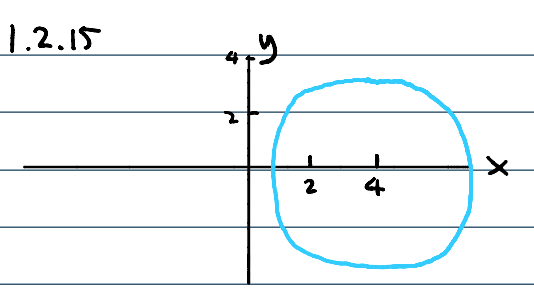
\includegraphics[width=2in]{1-2-15.png}
          \end{center}
    \item [1.2.16] $\abs{z+2+i}=1$\\
          \textbf{Answer: } Similar to the above, $\abs{z+2+i}=1$ is a circle of radius 1 centered at $(-2,-1)$.
          \begin{center}
              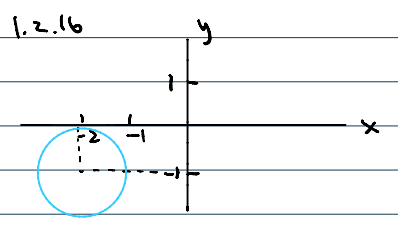
\includegraphics[width=2in]{1-2-16.png}
          \end{center}
    \item [1.2.34]
          \begin{itemize}
              \item [(a)] Use the triangle inequality to show that $\abs{z-1}\leq 2$ for $\abs{z}\leq 1$.
              \item [(b)] Explain your result in $(a)$ geometrically.
              \item [(c)] Is the upper bound in $(a)$ best possible?
          \end{itemize}
    \item [1.3.5] $-3-3i$\\
          \textbf{Answer: } $r=\sqrt{(-3)^2+(-3)^2}=3\sqrt{2}$; $\cos\theta=\frac{x}{r}=\frac{-3}{3\sqrt{2}}=-\frac{\sqrt{2}}{2},\sin\theta=\frac{y}{r}=\frac{-3}{3\sqrt{2}}=-\frac{\sqrt{2}}{2}\implies\theta=\frac{5\pi}{4}\implies\text{Arg }z=-\frac{3\pi}{4}$. Then $-3-3i=3\sqrt{2}(\cos(-\frac{3\pi}{4})+i\sin(-\frac{3\pi}{4}))$.
    \item [1.3.6] $-\frac{\sqrt{3}}{2}+\frac{i}{2}$\\
          \textbf{Answer: } $r=\sqrt{\frac{3}{4}+\frac{1}{4}}=1$; $\cos\theta=\frac{x}{r}=-\frac{\sqrt{3}}{2},\sin\theta=\frac{y}{r}=\frac{1}{2}\implies\theta=\frac{5\pi}{6}=\text{Arg }z$. Then $-\frac{\sqrt{3}}{2}+\frac{i}{2}=\cos\frac{5\pi}{6}+i\sin\frac{5\pi}{6}$.
    \item [1.3.21] $(1+i)^{30}$\\
          \textbf{Answer: } $(1+i)^{30}=\sqrt{2}^{30}(\cos\frac{\pi}{4}+i\sin\frac{\pi}{4})^{30}=2^{15}(\cos\frac{30\pi}{4}+i\sin\frac{30\pi}{4})=2^{15}(0+i)=2^{15}i$, so $\Re z=0$ and $\Im z=2^{15}$.
    \item [1.5.7] $e^{-1-i\frac{\pi}{6}}$\\
          \textbf{Answer: } $e^{-1-i\frac{\pi}{6}}=e^{-1}\cdot e^{-i\frac{\pi}{6}}=e^{-1}(\cos(\frac{-\pi}{6})+i\sin(\frac{\pi}{6}))=e^{-1}\cos(\frac{-\pi}{6})+ie^{-1}\sin(\frac{\pi}{6})$, so $a=e^{-1}\cos(\frac{-\pi}{6})$ and $b=e^{-1}\sin(\frac{\pi}{6})$.
    \item [P1] Let $z=x+iy$ be a complex number. Show that:
    \begin{itemize}
        \item [(a)] $\bar{\bar{z}}=z$
        \item [(b)] $\Re(z)=\frac{z+\bar{z}}{2}$
        \item [(c)] $\Im(z)=\frac{z-\bar{z}}{2i}$
    \end{itemize}
    \item [P2] Let $z_1=x_1+iy_1$ and $z_2=x_2+iy_2$ be complex numbers. Show that:
    \begin{itemize}
        \item [(a)] $\overline{z_1+z_2}=\overline{z_1}+\overline{z_2}$
        \item [(b)] $\overline{z_1z_2}=\overline{z_1}\cdot\overline{z_2}$
    \end{itemize}
    \item [P3]
    \begin{itemize}
        \item [(a)] Show that $\abs{z-4}\leq 6$ if $\abs{z-3i}\leq 1$
        \item [(b)] Show that $\abs{z-4}\geq 4$ if $\abs{z-3i}\leq 1$
        \item [(c)] Show that $\abs{\frac{1}{z-4}}\leq\frac{1}{2}$ if $\abs{z-1}\leq 1$
    \end{itemize}
\end{itemize}
\end{document}